\documentclass{article}

\usepackage[UTF8]{ctex}
\usepackage{placeins}
\usepackage{graphicx}
\usepackage{listings}
\usepackage{xcolor} % 添加 xcolor 宏包
\lstset{ %
language=matlab,                % choose the language of the code
basicstyle=\footnotesize,       % the size of the fonts that are used for the code
numbers=left,                   % where to put the line-numbers
numberstyle=\footnotesize,      % the size of the fonts that are used for the line-numbers
stepnumber=1,                   % the step between two line-numbers. If it is 1 each line will be numbered
numbersep=5pt,                  % how far the line-numbers are from the code
backgroundcolor=\color{white},  % choose the background color. You must add \usepackage{color}
showspaces=false,               % show spaces adding particular underscores
showstringspaces=false,         % underline spaces within strings
showtabs=false,                 % show tabs within strings adding particular underscores
frame=single,           % adds a frame around the code
tabsize=2,          % sets default tabsize to 2 spaces
captionpos=b,           % sets the caption-position to bottom
breaklines=true,        % sets automatic line breaking
breakatwhitespace=false,    % sets if automatic breaks should only happen at whitespace
escapeinside={\%*}{*)}          % if you want to add a comment within your code
}
\title{hw04\_MATLAB}
\author{3220103167 缪晨轩}
\date{\zhdate{2024/3/21}}

\begin{document}

\maketitle
    \section*{63(1)}
        \begin{lstlisting}[caption={题63(1)MATLAB代码}, label={lst:matlab}]
            syms t; % 声明符号变量

            % 定义函数
            f_t = sin(3*pi*(t - 2))/(pi*(t - 2)); % 原始函数

            % 计算傅里叶变换
            F_w = fourier(f_t); % 傅里叶变换

            % 计算最简形式的傅里叶变换
            F_w_simple = simplify(F_w); % 最简形式

            % 显示最简形式的傅里叶变换
            disp('傅里叶变换的最简形式:');
            disp(F_w_simple);

            % 绘制幅度谱和相位谱
            Fs = 1000; % 采样频率
            T = 1/Fs; % 采样间隔
            L = 2^nextpow2(Fs); % FFT长度
            t = (0:L-1)*T; % 时间向量
            f_t_values = sin(3*pi*(t - 2))./(pi*(t - 2)); % 计算函数值
            F = fft(f_t_values, L)/L; % 计算傅里叶变换

            % 计算频率轴
            frequencies = Fs*(0:(L/2))/L;

            % 绘制幅度谱和相位谱
            figure;

            subplot(2, 1, 1);
            plot(frequencies, 2*abs(F(1:L/2+1))); % 幅度谱
            title('Amplitude Spectrum');
            xlabel('Frequency (Hz)');
            ylabel('Magnitude');

            subplot(2, 1, 2);
            plot(frequencies, angle(F(1:L/2+1))); % 相位谱
            title('Phase Spectrum');
            xlabel('Frequency (Hz)');
            ylabel('Phase (radians)');

        \end{lstlisting}
        Answer: \[{e^{ - 2jw}}\left( {u\left( {w + 3\pi } \right) - u\left( {w - 3\pi } \right)} \right)\]
            \begin{figure}[h]
                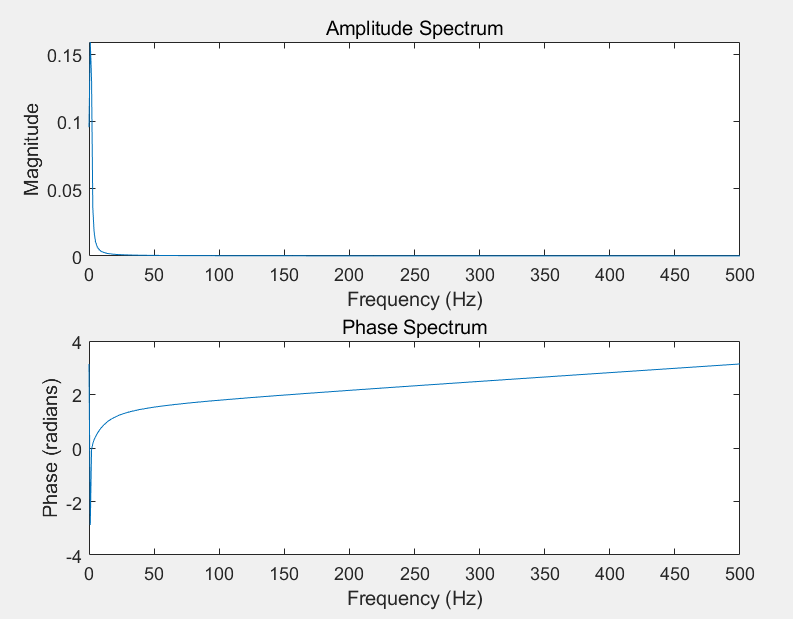
\includegraphics{63_1.png}
            \end{figure}
            \FloatBarrier
    \section*{63(2)}
        \begin{lstlisting}[caption={题63(2)MATLAB代码}, label={lst:matlab}]
            syms t; % 定义符号变量

            % 定义函数
            f_t = (sin(pi*t)/(pi*t))^2;

            % 计算傅里叶变换
            F_w = fourier(f_t);

            % 输出最简形式的傅里叶变换表达式
            F_w_simple = simplify(F_w);
            disp('最简形式的傅里叶变换表达式:');
            disp(F_w_simple);

            % 绘制幅度谱和相位谱
            Fs = 1000; % 采样频率
            T = 1/Fs; % 采样间隔
            L = 2^nextpow2(Fs); % FFT长度
            t = (0:L-1)*T; % 时间向量
            f_t_values = (sin(pi*t)/(pi*t)).^2; % 计算函数值
            F = fft(f_t_values, L)/L; % 计算傅里叶变换

            % 计算频率轴
            frequencies = Fs*(0:(L/2))/L;

            % 绘制幅度谱和相位谱
            figure;

            subplot(2, 1, 1);
            plot(frequencies, 2*abs(F(1:L/2+1))); % 幅度谱
            title('Amplitude Spectrum');
            xlabel('Frequency (Hz)');
            ylabel('Magnitude');

            subplot(2, 1, 2);
            plot(frequencies, angle(F(1:L/2+1))); % 相位谱
            title('Phase Spectrum');
            xlabel('Frequency (Hz)');
            ylabel('Phase (radians)');

        \end{lstlisting}
        Answer: \[ - \left( {F\left\{ {\frac{{\cos \left( {2\pi t} \right)}}{{{t^2}}}} \right\}} \right) + \frac{{\pi wsign\left( w \right)}}{{2{\pi ^2}}}\]
            \begin{figure}[h]
                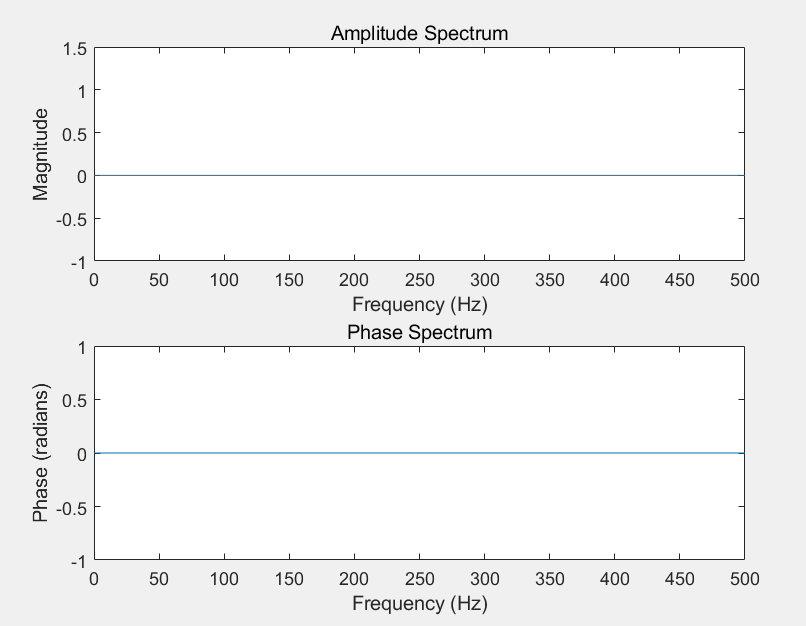
\includegraphics{63_2.png}
            \end{figure}
            \FloatBarrier
    \section*{64(1)}
        \begin{lstlisting}[caption={题64(1)MATLAB代码}, label={lst:matlab}]
            % 定义变量和参数
            syms t w0 w;  % 符号变量 w 和 w0

            % 定义频率域上的信号 X(w)
            X_w = heaviside(w + w0) - heaviside(w - w0);

            % 计算 X(w) 的傅里叶反变换
            x_t = ifourier(X_w, w, t);

            % 显示结果
            disp('Inverse Fourier Transform of X(w) =');
            disp(simplify(x_t));

        \end{lstlisting}
        Answer: \[\frac{{\sin \left( {t{w_0}} \right)}}{{t\pi }}\]
    \section*{64(2)}
        \begin{lstlisting}[caption={题64(2)MATLAB代码}, label={lst:matlab}]
            syms w w0 t; % 定义符号变量

            % 定义傅里叶变换
            X_w = dirac(w + w0) - dirac(w - w0);

            % 计算傅里叶反变换
            x_t = ifourier(X_w, w, t);

            % 输出傅里叶反变换表达式
            disp('傅里叶反变换表达式:');
            disp(x_t);

        \end{lstlisting}
        Answer: \[\frac{{{e^{ - it{w_0}}} - {e^{it{w_0}}}}}{{2\pi }}\]
    \section*{64(3)}
        \begin{lstlisting}[caption={题64(3)MATLAB代码}, label={lst:matlab}]
            syms w t; % 定义符号变量

            % 定义傅里叶变换
            X_w = 5*cos(2*w);

            % 计算傅里叶反变换
            x_t = ifourier(X_w, w, t);

            % 输出傅里叶反变换表达式
            disp('傅里叶反变换表达式:');
            disp(x_t);

        \end{lstlisting}
        Answer: \[\frac{{5\delta \left( {t - 2} \right) + 5\delta \left( {t + 2} \right)}}{2}\]
    \section*{64(4)}
        \begin{lstlisting}[caption={题64(4)MATLAB代码}, label={lst:matlab}]
            syms w t; % 定义符号变量

            % 定义傅里叶变换
            X_w = (heaviside(w) - heaviside(w - 1))*exp(-1i*w);
            
            % 计算傅里叶反变换
            x_t = ifourier(X_w, w, t);
            
            % 输出傅里叶反变换表达式
            disp('傅里叶反变换表达式:');
            disp(x_t);
            
        \end{lstlisting}
        Answer: \[ - \frac{{\left( { - \sin \left( {t - 1} \right) + i\cos \left( {t - 1} \right)} \right)/\left( {t - 1} \right) - i/\left( {t - 1} \right)}}{{2\pi }}\]
\end{document}